\documentclass[../main.tex]{subfiles}
\graphicspath{{\subfix{../media/}}}


\begin{document}

	\begin{figure}[h]
		\centering
		\begin{tikzpicture}

			\node[above, font=\large, align=center] at (7,6.6) {Evolutionary Process at Generation $\left(i\right)$};
		    % First box with randomly placed balls
		    \draw (0,0) rectangle (6,6);
		    \foreach \x/\y in {0.5/0.8, 1.2/2.5, 2.3/3.1, 3.1/1.4, 1.8/0.9, 
		                       4.2/5.1, 3.5/2.8, 2.7/4.5, 1.1/3.9,
		                       4.4/2.1, 3.3/4.7, 0.7/5.2, 1.9/2.3, 5.1/3.3}
		        \fill (\x, \y) circle (0.2);
		        
			% Arrow		
		    \draw[->, >=stealth, ultra thick] (6,3) -- (8,3) node[midway, above, text width=2.8cm, align=center] {Natural \\ Selection \\ Process};
		    \draw[->, >=stealth, ultra thick] (6,3) -- (8,3) node[midway, below, text width=2.8cm, align=center] {\scriptsize Survival of \\ The Fittest};

		    % Second box with randomly placed balls
		    \draw (8,0) rectangle (14,6);
		    \foreach \x/\y in {8.5/0.8, 9.2/2.5, 10.3/3.1, 11.1/1.4, 9.8/0.9, 
		                       12.2/5.1, 11.5/2.8, 10.7/4.5, 9.1/3.9,
		                       12.4/2.1, 11.3/4.7, 8.7/5.2, 9.9/2.3, 13.1/3.3}
		        \fill (\x, \y) circle (0.2);
		        
		    \foreach \x/\y in {8.5/0.8, 9.2/2.5, 10.3/3.1, 11.1/1.4, 9.8/0.9, 12.2/5.1}
			    \fill[red] (\x, \y) circle (0.2);

			% Arrow		
		    \draw[->, >=stealth, ultra thick] (11,0) -- (11,-2) node[midway, above, text width=2.8cm, align=center] {};


		    % Third box with randomly placed balls
		    \draw (8,-8) rectangle (14,-2);
		    \foreach \x/\y in {8.5/0.8-8, 9.2/2.5-8, 10.3/3.1-8, 11.1/1.4-8, 9.8/0.9-8, 12.2/5.1-8}
		        \fill[red] (\x, \y) circle (0.2);
		    \fill[red] (10.3, 3.1-8) circle (0.2);
		    		    
			% Arrow		
		    \draw[->, >=stealth, ultra thick] (8,-5) -- (6,-5) node[midway, above, text width=2.8cm, align=center] {Mutation};
		    \draw[->, >=stealth, ultra thick] (8,-5) -- (6,-5) node[midway, below, text width=2.8cm, align=center] {\scriptsize Offsprings \\ Children};
		    
		    % Fourth box with randomly placed balls
		    \draw (0,-8) rectangle (6,-2);
		    \foreach \x/\y in {0.5/0.8-8, 1.2/2.5-8, 2.3/3.1-8, 3.1/1.4-8, 1.8/0.9-8, 
		                       4.2/5.1-8}
		        \fill[red] (\x, \y) circle (0.2);
		        
		    \foreach \x/\y in {1.4/5-8, 1.4/0.7-8, 2.4/2.7-8, 2.0/2.0-8, 4.0/2.0-8, 0.9/0.9-8, 0.7/1.5-8, 0.6/3.5-8, 1.7/3.5-8, 2.7/3.4-8, 3.3/1.9-8, 5.2/0.8-8, 4.3/3.8-8, 
		                       3.2/5.1-8}
			    \fill[blue] (\x, \y) circle (0.15);


	        % Legend
		    \node[draw, fill=white] at (7,-9) {
		        \begin{tikzpicture}
		            \fill (0,0) circle (0.15);
		            \node[right] at (0.2,0) {Population};
		            \fill[red] (4,0) circle (0.15);
		            \node[right] at (4.2,0) {Offsprings};
		            \fill[blue] (8,0) circle (0.1);
		            \node[right] at (8.2,0) {Children};
		        \end{tikzpicture}
		    };
		\end{tikzpicture}
	    \caption{Evolutionary Process in Evolutionary Strategies Algorithm}
	\end{figure}
	
	
	\begin{figure}[h]
		\centering
	    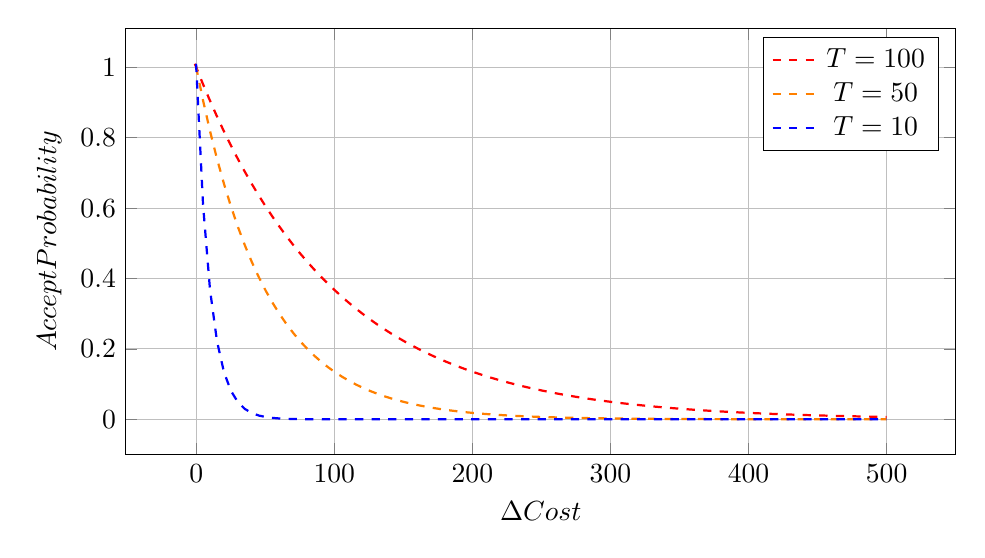
\begin{tikzpicture}
	        \begin{axis}[
	            xlabel = $\Delta \text{Cost}$,
	            ylabel = $\text{Accept Probability}$,
			  	width=\linewidth,
			  	height=7cm,
			  	grid=both,
	            declare function={
	                l0(\cost) = exp(-\cost/100);
	                l1(\cost) = exp(-\cost/10);
	            }
	        ]
	            
	            % Bases Functions
	            \addplot[thick, dashed, red, domain=-1:500, samples=100] {exp(-\x/100)};
	            \addplot[thick, dashed, orange, domain=-0.1:500, samples=100] {exp(-\x/50)};
	            \addplot[thick, dashed, blue, domain=-0.1:500, samples=100] {exp(-\x/10)};
					            
				\legend{$T=100$ , $T=50$, $T=10$}

	        \end{axis}
	    \end{tikzpicture}
	    \caption{Simulated Annealing Temperature }
	\end{figure}


	\SetKwComment{Comment}{/* }{ */}

	\begin{algorithm}
		\caption{Simulated Annealing Algorithm}\label{alg:two}
		\KwData{$T_i, \, x_i $}
		\KwResult{$x_{n} \gets \text{last solution candidate}$}\vspace{5pt}
		$T_0 \gets \text{initial temperature of cooling schedule}$\;
		$x_0 \gets \text{starting solution candidate}$\;\vspace{5pt}

		\For{$i \in \lbrace 0, \dots, n\rbrace$}{
		  $x_\text{neighbor} \gets \text{randomly sample a neighbor from } x_i \text{ neighborhood}$\\$\qquad\qquad\quad \text{ using uniform distribution}$\;
		  $\Delta \, cost \gets \text{compute cost difference between } x_\text{neighbor} \text{ and } x_i$\;\vspace{5pt}
		  \uIf{$\text{cost}(x_\text{neighbor}) \text{ is better than } \text{cost}(x_i)$}{
		    \textbf{Accept} $x_{i+1} \gets x_i$\;\vspace{5pt}
		  }
		  \uElseIf{$\text{cost}(x_\text{neighbor}) \text{ is worse than } \text{cost}(x_i)$}{\vspace{3pt}
		  	\eIf{\text{probability} $e^{-\Delta cost \,/\,T_i}$}{ 
		  		\textbf{Accept} $x_{i+1} \gets x_i$\;\vspace{5pt} 
		  	}
		  	{
		      	\textbf{Reject} \text{Do nothing};\vspace{5pt}
		  	}
		  }
		  }
	\end{algorithm}


\end{document}